\chapter{System Model}\label{ch:sysmodel}

As mentioned in Chapter \ref{ch:intro}, the goal of this thesis is to obtain measurement data from the MIMO setup. This collected experimental data will be applied to the machine learning model, that has been developed in parallel with this thesis. This chapter explains the relevant fundamentals of the LTE standard, which will be used as a basis for the experiments are described on a high level.

%\par
%
%In the following sections we would discuss the LTE frame structure and the relevant signalsthat are required for the collection of the data. The release of the LTE standard being used here is the Release 10.

\section{LTE}\label{sec:LTEProc}

LTE stands of Long Term Evolution and is a successor standard to UMTS. LTE was chosen as a standard to use for the communication system as it is currently widespread in the telecommunications industry and because of the integrated support of simulation environments like MATLAB, Labview and Simulink. LTE is a multicarrier approach for multiple access which uses Orthogonal Frequency-Division Multiple Access (OFDMA) in the physical layer. OFDMA uses multiple carriers (known as sub carriers) spaced equally apart and can transmit independent data streams on each sub carrier \cite{rohling}.

A LTE frame is commonly represented as a 2D time frequency grid, where the vertical axis represents the sub-carriers (Frequency) and the horizontal axis represents time. LTE also comes in 2 flavours Frequency Division Duplexing (FDD) and Time Division Duplexing (TDD). In this thesis the focus will be on FDD systems, which use seperate frequency bands, for uplink and for downlink data respectively. The advantage of an FDD system is that the uplink and downlink transmittion can happen simultaneously.

LTE has a certain predefined signalling symbol structure according to the standard \cite{3gpp36211}. In the following sections the frame structure and the different symbols in the LTE Frame shall be introduced.

\section{LTE Waveform Processing}\label{sec:LTE Waveform Processing}

\subsection{Transmission} \label{ssec:Transmission}

A dual antenna transmitter using a USRP software defined radio as mentioned in Section \ref{sec:USRP} is used as a transmitter. A modified version of the LTE Application framework with MIMO 2x2 extension is used to log the data. The transmitter USRP is connected to a Host PC using a 4-lane PCIe connection. This is necessary for the high data throughput exchanged between the host and the devices.

LTE has a standardized frame structure which is commonly represented as a 2D time frequency grid, where the vertical axis represents the sub-carriers and the horizontal axis represents time. LTE also uses a predefined signalling structure according to the standard \cite{3gpp36211}. In the following sections the frame structure and the symbols relavent to channel estimation shall be introduced.

\subsubsection{LTE Frame} \label{LTEFrame}

A single frame is 10\si{\milli\second} long and consists of 10 smaller units called subframe, each 1\si{\milli\second} long. A symbol is the smallest unit of time for an LTE system and one subframe has 14 such symbols each approximately 66.7\si{\micro\second} long. Scheduling is normally done on a subframe basis for both uplink and downlink communication.

LTE's time frequency grid contains many different signals each performing specific funtionality like broadcasting, control channel information, user data, among other functions.

For the purpose of channel estmation and the application as outline in this thesis, the most important signals are Primary Synchronisation Signal (PSS), Secondary Synchronisation Signal (SSS) and Cell Specific Reference Signal (CRS) which are described in detail in the subsequent sections.

\subsubsection {Primary Synchronisation Signal (PSS)} \label{sssec:PSS}
        OFDM is extremely time and frequency sensitive, hence it is very important to know the exact start of every frame. The PSS helps to achieve the synchronisation of the frame by using a specific sequence called the Zadoff-Chu sequence \cite{3gpp36211}.
        The Zadoff-Chu sequence has the property of constant amplitude zero autocorrelation waveform (CAZAC sequences) such that cyclically shifted versions of the waveform are orthogonal to original waveform. The sequence is described in Equation \ref{eq:ZCSeq} where {\em u}  can be 25,29 or 34 depending on the cell ID.
        The PSS is broadcast twice every radio frame and the symbols are identical each time.

\begin{equation} \label{eq:ZCSeq}
        d_u(n) =
        \begin{cases}
            \mathrm{e}^{-j\frac{\pi un(n+1)}{63}}       & \quad n=0,1,...,30\\
            \mathrm{e}^{-j\frac{\pi un(n+1)(n+2)}{63}} & \quad n=31,32,...,61
        \end{cases}
\end{equation}

\subsubsection{Secondary Synchronisation Signal (SSS)} \label{sssec:SSS}
        The SSS is a 62 bit BPSK modulated pseudo random sequence \cite{3gpp36211}. It is broadcast twice in a frame once in subframe 0 and once in subframe 5, one symbol before the PSS. The 2 sequences of transmission in a frame are different so that the UE can identify which position in the frame the synchronisation happens.

\subsubsection{Cell Specific Reference Signal (CRS)} \label{sssec:CRS}
        As mentioned in Chapter \ref{ch:intro} the channel needs to be estimated in order to reverse the channel propogation effects. With the help of CRS the channel can be estimated by placing equally spaced reference symbols every 6 subcarriers starting from subcarrier 2 on symbols 1, 8, 15, etc... and every 6 subcarriers starting from subcarrier 5 on symbols 5, 12, 19, etc...\cite{3gpp36211}. The signals received by the UE and the channel effects are inferred based on amplitude damping and phase shift. Placing the signals in the above defined spacing gives the best coverage to interpolate over in time and frequency.

        The signals to be placed on the grid are decided by the Equation \ref{eq:CRS} as shown below, with the parameters defined in Table \ref{tab:CRSParam} \cite{3gpp36211}.
        \begin{equation} \label{eq:CRS}
            r_{l,n_s}(m) = \frac{1}{\sqrt{2}}(1-2{\cdot}c(2m)) + j\frac{1}{\sqrt{2}}(1-2{\cdot}c(2m+1)),\ m=0,1,...,2N_{RB}^{max,DL}-1
        \end{equation}

        \begin{table}[H]
            \begin{center}
                \begin{tabular}{|l|l|}
                    \hline
                    Parameter& Description\\ \hline
                    $c(m)$& Pseudo Random Sequence defined in \cite{3gpp36211}\\ \hline
                    $N_{RB}^{max,DL}$& Maximum number of Downlink resources blocks\\ \hline
                    $n_s$& Slot number in the frame\\ \hline
                    $l$& OFDM Symbol number in the frame\\
                    \hline
                \end{tabular}
                \caption{Parameter definitions for evaluating CRS Symbols}
                \label{tab:CRSParam}
            \end{center}
        \end{table}

        In the case of multiple antennas, each antenna port has a dedicated CRS slots and have their corresponding positions on the OFDM time/frquency grid as shown in Figure \ref{fig:CRSMultiAntenna}. These CRS signals for different antennas are signaling overheads, which implies that they cannot be used for data transmission. On the receiver end this particular symbol is decoded and the channel estimate is calculated for the respective transmit antenna.

\begin{figure}[H]
    \begin{center}
        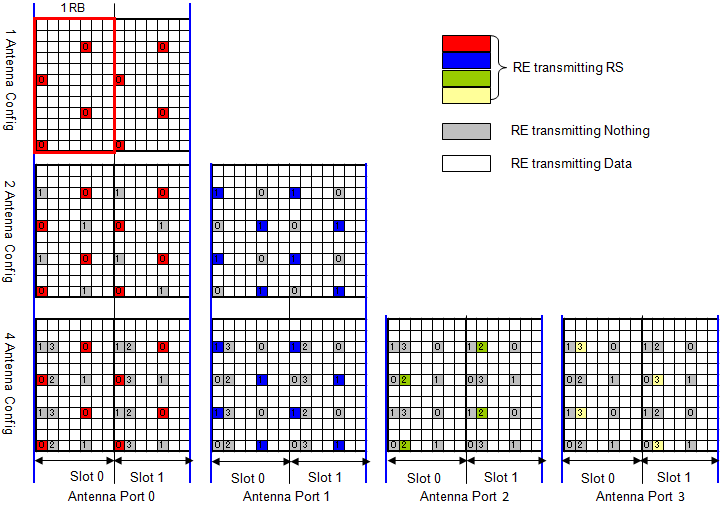
\includegraphics[width=\linewidth]{images/CRSMultiAntenna.png}
        \caption{Reference Signal layout for multi antenna configurations of 1,2 and 4 antenna systems in LTE}
        \label{fig:CRSMultiAntenna}
    \end{center}
\end{figure}


\subsubsection{Final Waveform}
All the signals mentioned in Section \ref{LTEFrame} are generated in Labview along with other signals that are not mentioned here due to the complexity are generated using the LTE Application Framework Software and arranged in a 2D grid of frequency and time as shown below in Figure \ref{fig:RBSignals}. The CRS for a 2 antenna system are placed every 6 subcarriers in the frequency domain and every 3 or 4 time symbols apart, according to the position on the grid. Where as the PSS and SSS only repeat every 5 subframes.

\begin{figure}[H]
    \begin{center}
        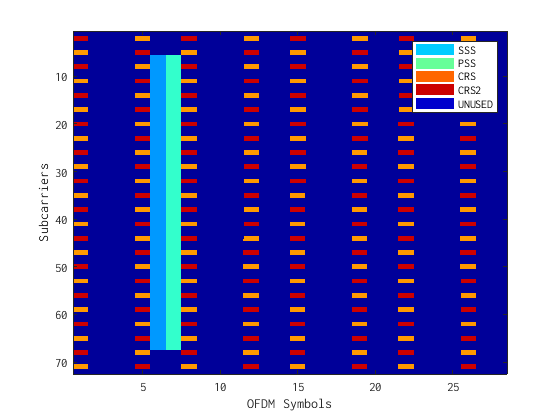
\includegraphics[width=10cm]{images/FrameLegend.png}
        \caption{Resource Block Grid for 2 sub frames}
        \label{fig:RBSignals}
    \end{center}
\end{figure}

One of the disadvantages of using OFDM in the physical layer is the high peak to average power ratio (PAPR) of the signal. High PAPR translates to high fidelity requirements of power amplifiers on the transmitter side. It also induces non-linear distortions to the signal \cite{rohling}. To ensure that the PAPR of the signal is as low as it can be, random QPSK symbols are transmitted on the unused slots instead of 0s.

\subsection{Reception}

For the LTE receiver processing a USRP with 2 antennas acquires the RF data from both ports and processes the data in the FPGA in real time. The data requested by the host is then forwarded to it using the high speed PCIe interface. A more in depth explaination of the receiver processing is explained in Chapter \ref{ch:ExSetup}.

The channel estimation data is forwarded from the FPGA IQ processing engine to the host which is then logged to a TDMS file (NI propriotory format) and post processed to extract samples for the purpose of the experiments. The main steps of the DL receiver processing once enough samples have been captured are the following.


\subsubsection{Carrier Offset Estimation and Correction}
OFDM is extremely senstive to frequency shifts in the received signal. In the case that the receiver or transmitter center frequency clock was not accurate enough, the frequency shift needs to be estimated and corrected. This is the very first step before processing the baseband waveform.

\subsubsection{Frame synchronisation}
As mentioned in Section \ref{LTEFrame} the synchronisation is a very important part of knowing where the LTE frame begins. This is done by correlating the received signal with the known Zadoff Chu Sequence and to look for the peak. Figure \ref{fig:PSSCorr} shows an example correlation of a Zadoff Chu sequence and a received signal containing 307200 samples in total amounting to 2 frames of a 10\si{\mega\hertz} Bandwidth LTE signal. 4 peaks are to be expected here as there are 2 frames, each containing 2 PSS sequences.

\begin{figure}[H]
    \begin{center}
        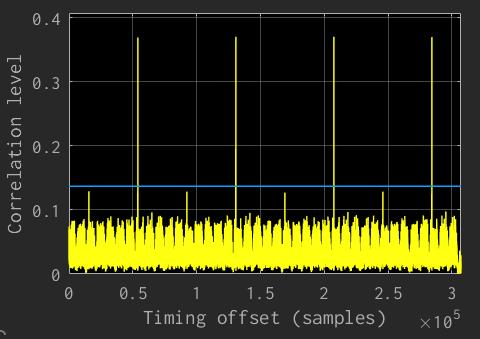
\includegraphics[width=9cm]{images/PSSCorrelation.jpg}
        \caption{PSS Correlation}
        \label{fig:PSSCorr}
    \end{center}
\end{figure}

\subsubsection{Channel Estimation}

Once the frame has been demodulated and the 2D OFDM grid has been obtained, the channel can be estimated based on the original pilot symbols structure known to the receiver, hence the phase and amplitude of the particular sub carrier can be obtained. A linear interpolator is applied in the frequency axis to interpolate the channel estimate from 200 subcarriers to 1200 subcarriers(for a full bandwidth system) and a zero order hold is used in the time axis until the next pilot symbol in the time domain is encountered. The details are explained in the Chapter \ref{ch:ChEst}.


\subsection{Antenna}
The analog time domain signal is transmitted from the USRP (Section \ref{sec:USRP}) over the air using a Triband antenna. For the setup an omni directional Antenna from NI capable of transmitting and receiving around frequencies of 144, 400 or 1200 \si{\mega\hertz} is used for the transmitter and receiver as shown in Figure \ref{fig:USRPAnt}.

\begin{figure}[H]
    \begin{center}
        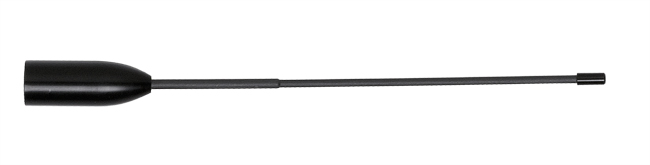
\includegraphics[width=7cm]{images/vert400.jpg}
        \caption{Narrowband Omnidirectional Antenna used for transmitting and receiving the LTE Signals}
        \label{fig:USRPAnt}
    \end{center}
\end{figure}
